\subsection{Introduction}

There are many multiple precision (MP) packages available to
the scientific and engineering community.
Each package has individual strengths within its range
of application. However, most MP packages lack a uniform interface
for high precision algorithm design. They also offer little or
no special function support. Also, many MP packages have
limited portability. There is no portable standalone C++ system
which offers a wide variety of high precision special functions
and handles large function parameters.

The \efloat\ system (extended float) not only addresses these weaknesses
but also significantly advances MP technology. It uses several 
MP packages and provides a uniform C++ interface for high precision
algorithm design, independent of the underlying MP implementation.
In addition, \efloat\ supports a large collection
of high performance MP functions which are
entirely portable, solidly designed and can be used with any
suitably prepared MP type. Furthermore, the \efloat\ system
provides software interfaces for seamless interoperability
with other high level languages.
No MP system other than \efloat\ offers such a high degree
of portability, such a wide range of functions, and such
a rich selection of powerful interoperabilities.
The \efloat\ library can be used for a variety of
purposes such as high precision function evaluation,
numerical verification of compilers, function libraries or
other computational systems as well as investigations of
compiler quality, optimization methods and computer hardware.

\efloat\ is unique because it is designed from the ground up utilizing
generic and object--oriented design methods to create an efficient and
flexible numerical software architecture
\cite{coplien:textbook}, \cite{vandevoorde:textbook}, \cite{yang:textbook}.
The standard containers and algorithms of the C++ STL and TR1 are
consistently used to reduce programmatic complexity \cite{becker:textbook},
\cite{isoiec14882:textbook}, \cite{isoiec19768:textbook}, \cite{josuttis:textbook}.
Static and dynamic polymorphism are used to implement a standardized
interface to MP types allowing for the interchangeable use of different
MP implementations.

\efloat\ is written in the C++ language making broad use of the
C++ core language, much of the STL and some of TR1,
as specified in ISO/IEC 14882:2003
and ISO/IEC 19768:2007 \cite{isoiec14882:textbook,isoiec19768:textbook}.
It is emphasized that the C++ compiler must closely adhere to
these standards in order to successfully compile and link \efloat.
The source codes have been implemented according to safe programming
practices and reliability standards originating from the automotive industry
\cite{misra:misrac,misra:misracpp}.
A great effort has been invested in advanced C++ optimization techniques
in order to improve system performance.
Generic and object--oriented programming methods have been used
to create an efficient and flexible numerical software architecture.
In addition, consistent use of standard containers and algorithms of the
STL and TR1~\cite{josuttis:textbook,becker:textbook} has significantly
reduced and evenly distributed the computational complexities
of the entire program.

Advanced programming techniques have been used to implement
interfaces to other high level languages, including the
Microsoft{\footnotesize {\textregistered}}~CLR,
Python, Iron\-Python and Wolfram's \mathematica\
(see \cite{isoiec23271:textbook,microsoft:clr,python:website,foord:textbook,ironpython:website,wolfram:textbook}).
This means that it is possible to combine the calculating power of several systems
to obtain a hybrid system which is more powerful than either one of its parts.
For example, \efloat\ can be used with the C\# language~\cite{isoiec23270:textbook},
targeting the CLR in the
Microsoft{\footnotesize {\textregistered}}.NET Framework.
This exposes the efficient calculating power of \efloat\ to the high level
graphical--user--interface (GUI) design regime of C\# in the CLR.
At the same time the GUI design is separated from complex MP algorithms.
This is a very powerful hybrid system based on effective distribution of
computational complexity.

The \efloat\ software project consists of approximately 110 manually written
source files with $\sim$20,000 lines of code in addition to about 20 automatically
generated files with $\sim$200,000 lines of code.
The source codes of \efloat\ are implemented in accordance with safe programming
practices and reliability standards originating from the automotive industry
\cite{misra:misrac}, \cite{misra:misracpp}.

The \efloat\ source code is released under the `Boost Software License' (BSL)
from boost \cite{boostlic:website}. Unlike the the `General Public License' (GPL)
from GNU \cite{gnulic:website}, the BSL permits the creation of works derived from \efloat\
for any commercial, or non-commercial, or non-profit use with no legal requirement
to release the \efloat\ source code \cite{boostlic:website}.

\subsection{Configurations}

\begin{table}[h]\noindent
\begin{center}
\renewcommand{\arraystretch}{1.05}
\begin{tabular}{c|c|c|c}

Config
            & \efloatclass\ Class
            & Capabilities
            & Dependencies \\

\hline

\multirow{2}{*}{efx}
            & \multirow{2}{*}{\efxefloatclass}
            & functions, algorithm design,
            & \multirow{2}{*}{---} \\

\ %space
            & \ %space
            & test and benchmark
            & \\

\hline

gmp
            & \gmpefloatclass\
            & ''$\quad\quad$''
            & GMP library \\

\hline

\multirow{2}{*}{mpfr}
            & \multirow{2}{*}{\mpfrefloatclass}
            & \multirow{2}{*}{''$\quad\quad$''}
            & GMP library, \\

\ %space
            & \ %space
            & \ %space
            & MPFR library \\

\hline

\multirow{2}{*}{f90}
            & \multirow{2}{*}{\mpfrefloatclass}
            & \multirow{2}{*}{''$\quad\quad$''}
            & {\courier{REAL(KIND\ensuremath{=}16)}} wrap, \\

\ %space
            & \ %space
            & \ %space
            & Fortran run--time libraries \\

\hline

\multirow{3}{*}{pyd}
            & \multirow{3}{*}{any \efloatclass}
            & functions, algorithm design,
            & those of its {\courier{e{\ttfamily\underline\ }float}} type, \\

\ %space
            & \ %space
            & rapid prototyping,
            & {\courier{boost.python}} library, \\

\ %space
            & \ %space
            & high level Python scripting
            & Python library \\

\hline

\multirow{4}{*}{clr}
            & \multirow{4}{*}{any \efloatclass}
            & functions, algorithm design,
            & \ \\

\ %space
            & \ %space
            & rapid prototyping,
            & those of its {\courier{e{\ttfamily\underline\ }float}} type, \\

\ %space
            & \ %space
            & high level scripting,
            & common language runtime \\

\ %space
            & \ %space
            & CLR GUI development
            & \ \\

\hline


\multirow{2}{*}{cas}
            & \multirow{2}{*}{any \efloatclass}
            & \multirow{2}{*}{computer algebra interoperability}
            & those of its {\courier{e{\ttfamily\underline\ }float}} type, \\

\ %space
            & \ %space
            & \ %space
            & computer algebra system \\

\hline
\end{tabular}
\vspace{2.0mm}
\caption{The system configurations of \efloat\ are shown.}
\label{table:systemconfigs}
\end{center}
\end{table}



The \efloat\ system supports a variety of configurations
using several \efloatclass\ classes
as well as other libraries and systems.
These are shown in Table~\ref{table:systemconfigs}.
Details about the capabilities and dependencies of the
configurations are also included in the table.

\pagebreak

\subsection{The \efloathyperref\ System Architecture}\label{sec:architecture}

\begin{figure*}[p]
\centering
\framebox{\hspace{2.0mm}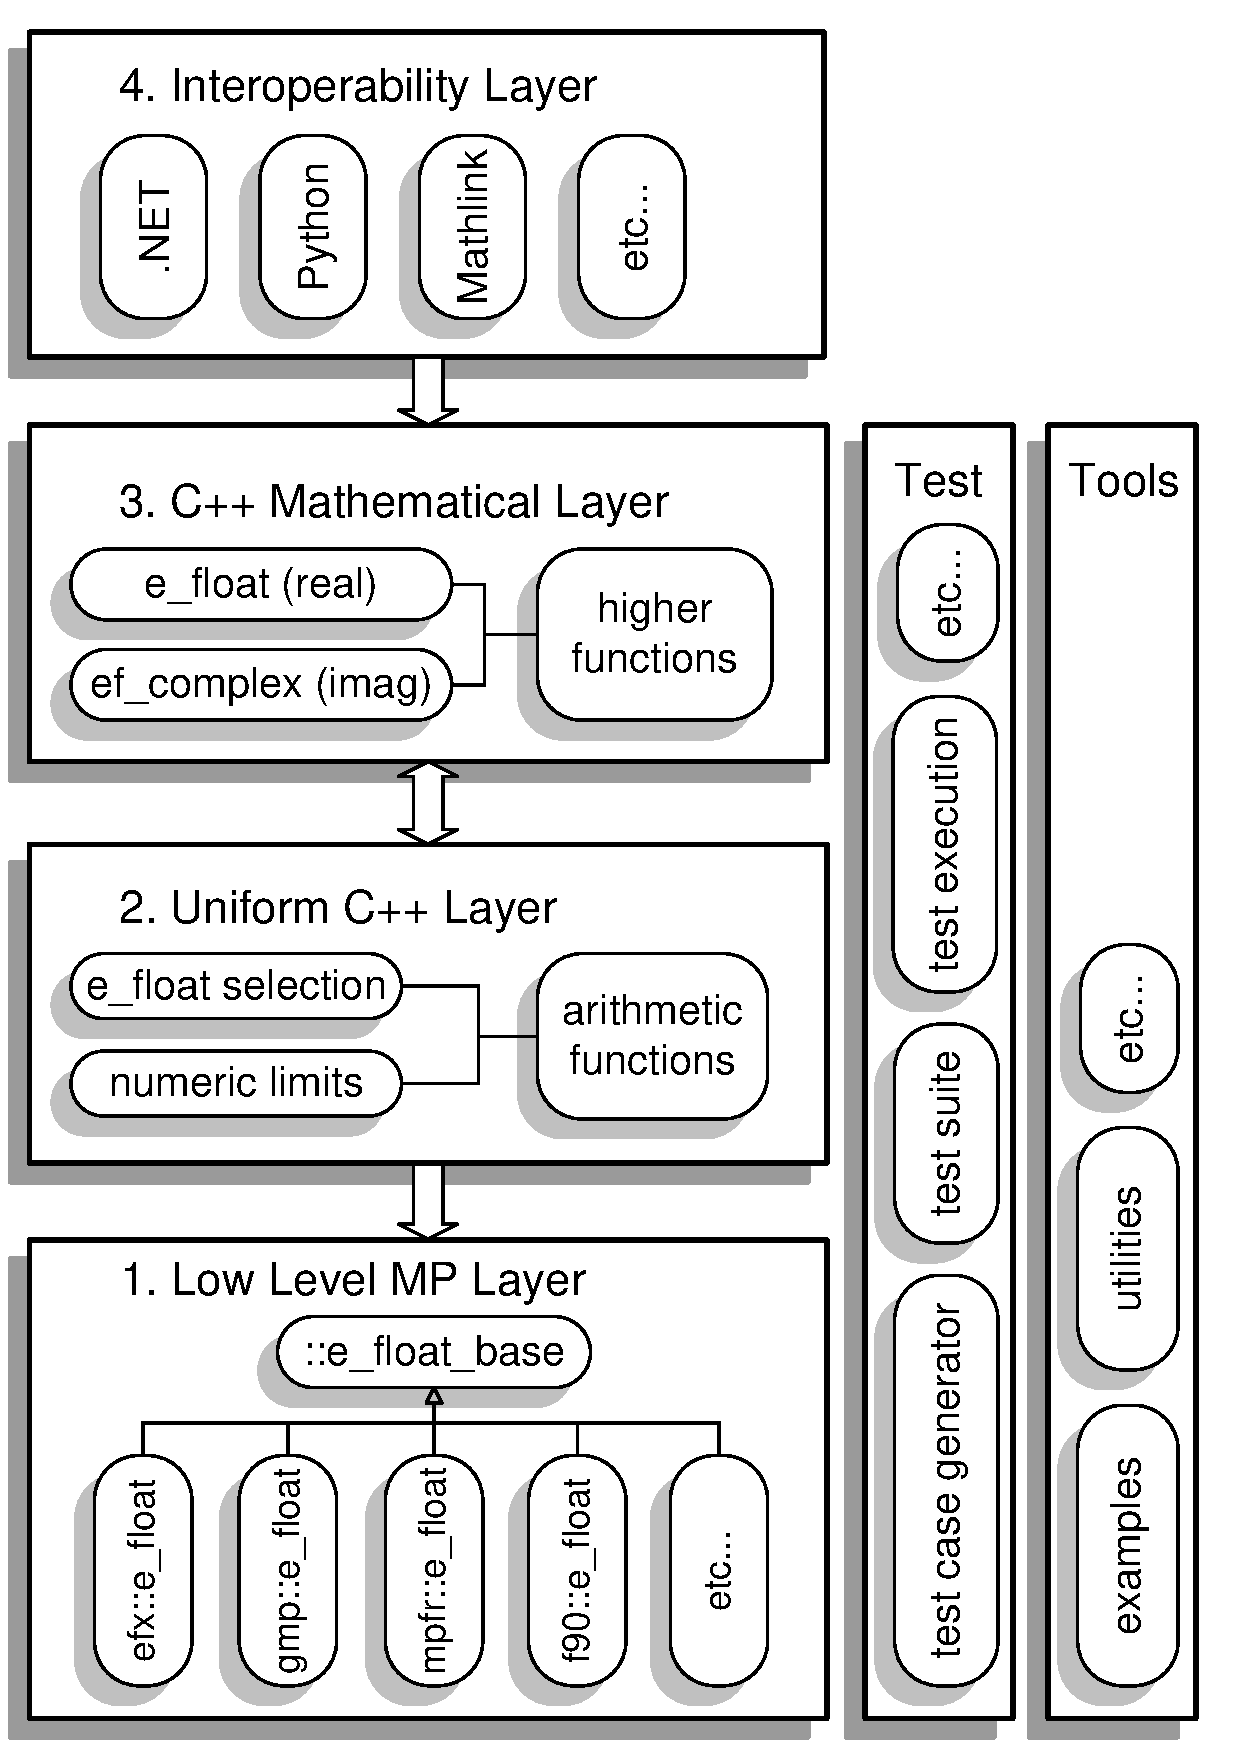
\includegraphics[width=16.0cm]{e_float_architecture.pdf}}
\vspace{2.0mm}
\caption{The \efloat\ system architecture is shown.}
\label{figure:architecture}
\end{figure*}

The \efloat\ system architecture is robust and flexible.
With this architecture, both the integration of other MP types as well as
the addition of more functions and interoperabilities can be done with ease. 
The system architecture is shown in Figure~\ref{figure:architecture}.
It has four layers and two additional
blocks, the test block and the tools block. Layers $1$--$4$ have successively
increasing levels of abstraction. They build up very high level
functionalities in a stable, stepwise fashion.
Note that ``{\emph e}{\ttfamily{\underline\ }}{\emph{float}}''
is not only the name of the system but also the name of several
\efloatclass\ classes.

Layer~$1$, the low level MP layer, ensures that each
implementation--dependent, possibly non--portable MP implementation
is suitably prepared to conform with the C++ class requirements of Layer~$2$.
Each individual MP type is encapsulated within a specific
\efloatclass\ C++ class,
each one of which defined within its own unique name\-space.
For example, classes such as
{\courier{efx::e{\ttfamily\underline\ }float}},
{\courier{gmp::e\underline\ float}} and others are implemented.
Each of these classes is derived from a common abstract
base class called {\courier{::e{\ttfamily\underline\ }float{\ttfamily\underline\ }base}}.
The abstract base class defines public and pure virtual functions
which implement arithmetic primitives such as self--multiplication,
self--compare, special numbers like NaN, and string operations.
These arithmetic primitives fulfill the requirements necessary for
elementary mathematics. They simultaneously conform with Layer~$2$.
Thus, via inheritance and implementation of virtual functions,
each individual \efloatclass\
class supports elementary mathematics and also complies with Layer~$2$.

Some MP types include their own versions of various functions.
Layer~$1$ accommodates this with the
``{\emph{has--its--own}}''--mechanism. This mechanism allows the
C++ interface of a given MP type to use the MP's own
algorithm for a particular function.
It uses virtual Boolean functions prefixed with
``{\courier{has{\ttfamily\underline\ }its{\ttfamily\underline\ }own}}''.
For example,
{\courier{has{\ttfamily\underline\ }its{\ttfamily\underline\ }own{\ttfamily\underline\ }sin}}
returns {\courier{true}} in order to use the MP's own implementation
of $\sin(x)$, $x$$\,\in$$\,\mathbb{R}$.
The performance of a specific MP class can be optimized
by selectively activating these functions.
MPFR~\cite{33:2:1} has its own implementations of most elementary functions
and several higher transcendental functions. The elementary functions
are quite efficient and these are, in fact, used to optimize the
performance of {\courier{mpfr::e{\ttfamily\underline\ }float}}.

Layer~$2$ implements the uniform C++ interface.
The \efloatclass\ type from layer~$1$, which will be used in the
project configuration, is selected with a
compile--time option. The functions of this \efloatclass\
class are used to implement all arithmetic operations,
numeric limits and basic I/O mechanisms.
Thus, layer~$2$ provides a uniform C++ interface which is
generic and fully equipped with all the basic functions
necessary for high level MP algorithm design in a C++ environment.

Layer~$3$ is the C++ mathematical layer.
It adds the class {\courier{ef{\ttfamily\underline\ }complex}},
{\emph{i.e.}} the complex data type. 
This layer uses both the selected \efloatclass\
type as well as {\courier{ef{\ttfamily\underline\ }complex}}
to implement \efloat 's rich collection of elementary functions and higher
transcendental functions.

Layer~$4$, the interoperability user layer, exposes all of the
functions and capabilities of layers~$2$ and $3$ to other
high level languages. Marshaling techniques~\cite{richterclr:textbook}
are used to create managed C++ classes and wrapper functions
which embody the full functionality of layers~$2$ and $3$.
These are compiled to a single CLR assembly which can be used with
all Microsoft{\footnotesize {\textregistered}} CLR
languages including C\#, managed C++/CLI, Iron\-Python, {\emph{etc}}.
Compatibility with the
Microsoft{\footnotesize {\textregistered}}.NET Framework~$3$.$5$ has been tested.
Another interoperability employs the {\courier{boost.py\-thon}}
library~\cite{boostpython:website} to
expose the functionality of layers~$2$ and $3$ to Python.
Compatibilities with Python~$2$.$6$.$4$ and boost~$\geq\,1$.$39$
have been tested.

Another layer~$4$ interoperability targets \mathematica.
A sparse architecture has been developed to create a generic interface
for interacting with computer algebra systems. The compatibility
of this interface with \mathematica~$7$.$1$ has been tested.
The interoperabilities of layer~$4$ are very powerful mechanisms
based on highly advanced programming techniques.
They can be used for very high level designs such as
scripting, rapid algorithm prototyping and result visualization.

The test block contains several hundred automatically
generated test files which have been specifically designed to test all
algorithms and convergence regions of the entire \efloat\ system.
The test block includes an automatic test execution system and an automatic
test case generator. This block allows for fully reproducible automated
testing of the system.

The tool block contains a variety of utilities and examples.
The utilities predominantly consist of generic templates
for standard mathematical operations such as numerical differentiation,
root finding, recursive quadrature, {\emph{etc}}.
The examples show practical, non--trivial
uses of the \efloat\ system involving both high level algorithm design
as well as interoperability.

The \efloat\ architecture exemplifies how layered
design can be leveraged to find the right granularity to distribute
a very large computational complexity among smaller constituents
which have manageable software scope.
For example, there are vast software distances
between the hand--optimized assembler routines of
GNU MP~\cite{gmp:website} and, for example, the Hurwitz zeta function,
or a high level GUI in C\#.
The \efloat\ architecture elegantly navigates
these distances to build up high level functionalities in
a controlled, stepwise fashion.

The \efloat\ system architecture is a significant technological
milestone in MP programming technology. While other MP packages do sometimes
provide a specialized C++ interface for their own specific implementations,
they are mostly incompatible with each other.
However, \efloat 's uniform C++ layer creates a
generic interface which can be used with any underlying MP type.
Assuming that a given MP type can be brought into conformance with layer~$2$,
it can be used in a portable fashion with all of \efloat 's capabilities
including arithmetic, elementary functions, special functions, interoperabilities,
automatic tests, utilities, and additional user--created extensions.

\pagebreak

\subsection{MP Types}

\begin{table}[ht]\noindent
\begin{center}
\renewcommand{\arraystretch}{1.20}
\begin{tabular}{c|l|c|c}

Class Name
            & Internal Representation
						& Digits
						& Padding \\

\hline

\multirow{4}{*}{{\courier{efx::e{\ttfamily\underline\ }float}}}
            & data: {\courier{UINT32}} base--$10^{8}$ array
						& \multirow{4}{*}{$30$--$300$}
						& \multirow{4}{*}{$15$\%} \\

\ %space
            & Boolean negative sign
            & \ %space
						& \ \\

\ %space
            & {\courier{INT64}} base--10 exponent
            & \ %space
						& \ \\

\ %space
            & floating point class (finite, NaN, {\emph{etc}}.)
            & \ %space
						& \ \\

\hline

\multirow{2}{*}{{\courier{gmp::e{\ttfamily\underline\ }float}}}
            & data: GMP's type {\courier{::mpf{\ttfamily\underline\ }t}}
						& \multirow{2}{*}{$30$--$300$}
						& \multirow{2}{*}{$15$\%} \\

\ %space
            & floating point class (finite, NaN, {\emph{etc}}.)
            & \ %space
						& \ \\

\hline

{\courier{mpfr::e{\ttfamily\underline\ }float}}
            & data: MPFR's type {\courier{::mpfr{\ttfamily\underline\ }t}}
						& $30$--$300$
						& $15$\% \\

\hline

{\courier{f90::e{\ttfamily\underline\ }float}}
            & data: Fortran's type {\courier{REAL(KIND\ensuremath{=}16)}}
						& $\sim$$\,30$
						& $4$--$5$ digits \\

\hline

\end{tabular}
\vspace{2.0mm}
\caption{The MP classes in \efloat\ are shown. Details about the internal representation
as well as the digit range and the added internal extra digits ({\emph{i.e.}} the padding) are given.}
\label{table:mpclasses}
\end{center}
\end{table}



Four MP types have been selected for inclusion in \efloat.
These are listed in Table~\ref{table:mpclasses}.
The table also includes information about the internal
representations of the individual MP classes and
their digit ranges.
The three main \efloatclass\ classes are
\efxefloatclass, \mpfrefloatclass\ and \gmpefloatclass.
They are designed for high precision calculations with large
exponent range.

GNU MP and MPFR have been included
because of their high performance, their general acceptance
in the scientific community and their widespread availability
(at least for Unix/Linux--GNU systems). Unfortunately,
these libraries are not easily ported to compiler and
build systems other than GCC and GNU\-make.
However, for the \efloat\ development GNU MP~$4$.$2$.$4$
and MPFR~$2$.$4$.$1$ have been ported to
Microsoft{\footnotesize {\textregistered}}
Visual Studio{\footnotesize {\textregistered}} 2008,
based in part on Glad\-man's~\cite{gladman:ports} port.

A new MP type called EFX, {\emph {extended--float--x}}, has been created for
the \efloat\ system. It is written entirely in C++ and uses
base--$10^{8}$ data elements. Since GNU MP and MPFR use more
efficient base--$2^{n}$ data elements and because they take advantage
of hand--optimized assembler for the most time--critical inner loops,
EFX does not quite reach the performance of either GNU MP or MPFR.
However, EFX has other advantages --- a base--$10$ representation as
well as a data field which is created on the stack, not using dynamic
memory allocation. Therefore, the base--10 numerical value can be viewed
in a human recognizable form with a graphical debugger,
without awkward print operations or code modifications.
This makes EFX well suited for algorithm development. EFX has been used
for all early algorithm prototyping during the \efloat\ development.

The final MP type is called F90. It uses a skinny For\-tran~$90$/C++
layer to wrap the Fortran quadruple--precision data type
{\courier{REAL(KIND\ensuremath{=}16)}}.
The range of this MP type is limited to that of
the Fortran type --- about 30 digits of precision with an exponent
of about $\pm\,4000$. Due to its limited range, \forefloatclass\
only passes about $75$\% of the test cases defined in
the test suite. If this range sufficient
for the application, then \forefloatclass\ is extremely fast
because it uses a native data type.


